\documentclass{beamer}
\usepackage{HECbeamer}
% \usepackage{pgfpages}
% \pgfpagesuselayout{4 on 1}[letterpaper, landscape, border shrink=5mm]
\title[\color{white}{MATH 60604A \S~5f - Other covariance models}]{\texorpdfstring{MATH 60604A \\Statistical modelling \\ \S~5f - Other covariance models}{MATH 60604A \\Statistical modelling \\ \S~5f - Other covariance models}}
\author{Léo Belzile}
\institute{HEC Montréal\\
Department of Decision Sciences}
\date{} 

\begin{document}
\frame{\titlepage}



\begin{frame}[fragile]
\frametitle{Heterogeneous autoregressive structure}
\bi
\item With longitudinal data, it often happens that the variance of the observations is a function of the measurement time. 
\item Several covariance structures in \code{proc mixed} have a ``heterogeneous'' version, i.e., where the variances can be different for different time measures.
\item The heterogeneous autoregressive model,
$\mathsf{ARH}(1)$, has the same correlation structure as $\mathsf{AR}(1)$. Its covariance matrix is
\[
\bs{\Sigma}_i=
  \begin{pmatrix}
   \sigma^2_1 & \sigma_1\sigma_2\rho & \sigma_1\sigma_3\rho^2 & \sigma_1\sigma_4\rho^3 & \sigma_1\sigma_5\rho^4\\
    \sigma_2\sigma_1\rho & \sigma^2_2 & \sigma_2\sigma_3\rho & \sigma_2\sigma_4\rho^2 & \sigma_2\sigma_5\rho^3\\
    \sigma_3\sigma_1\rho^2 & \sigma_3\sigma_2\rho & \sigma_3^2 & \sigma_3\sigma_4\rho & \sigma_3\sigma_5\rho^2\\
       \sigma_4\sigma_1\rho^3 & \sigma_4\sigma_2\rho^2 & \sigma_4\sigma_3\rho & \sigma^2_4 & \sigma_4\sigma_5\rho\\
       \sigma_5\sigma_1\rho^4 & \sigma_5\sigma_2\rho^3 & \sigma_5\sigma_3\rho^2 & \sigma_5\sigma_2\rho & \sigma_5^2
  \end{pmatrix}.
\]
\item Instead of assuming a common variance $\sigma^2$ for all time measures, the $\mathsf{ARH}(1)$ model allows for different variance $\sigma_j^2$ at time $j$.
\ei
\end{frame}


\begin{frame}[fragile]
\frametitle{Syntax for adjusting the heterogeneous $\mathsf{ARH}(1)$ model}
\begin{tcolorbox}[colback=white, colframe=hecblue, title=\SASlang{} code to fit heterogeneous $\mathsf{ARH}(1)$ model]
\begin{verbatim}
proc mixed data=revenge method=reml;
class id tcat;
model revenge = sex age vc wom t / solution;
repeated tcat / subject=id type=arh(1) r=1 rcorr=1;
run;
\end{verbatim}
\end{tcolorbox}
\end{frame}

\begin{frame}[fragile]
\frametitle{Correlation and covariance matrices for subject 1 ($\mathsf{ARH}(1)$)}
\begin{center}
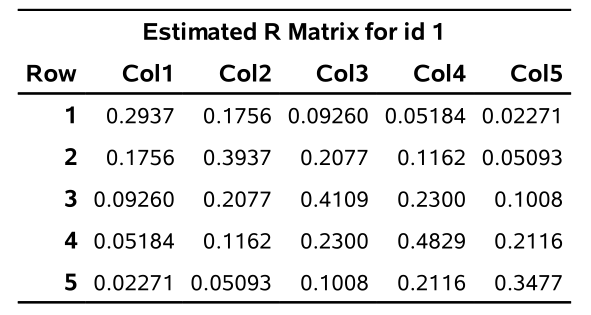
\includegraphics[width = 0.45\linewidth]{img/c5/slides6-e18a}
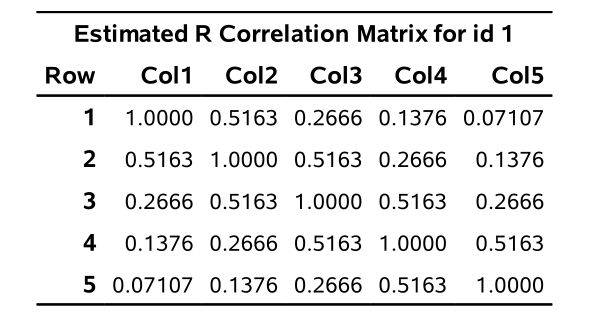
\includegraphics[width = 0.45\linewidth]{img/c5/slides6-e18b}

\end{center}
\bi
\item The covariance matrix shows that the variance of the observations is different for each measurement time
\item The correlation matrix shows, as for the $\mathsf{AR}(1)$ structure, that the correlation between two observations decreases over time.
\ei
\end{frame}

\begin{frame}[fragile]
\frametitle{Covariance parameters estimates of $\mathsf{ARH}(1)$ model}
\begin{center}
 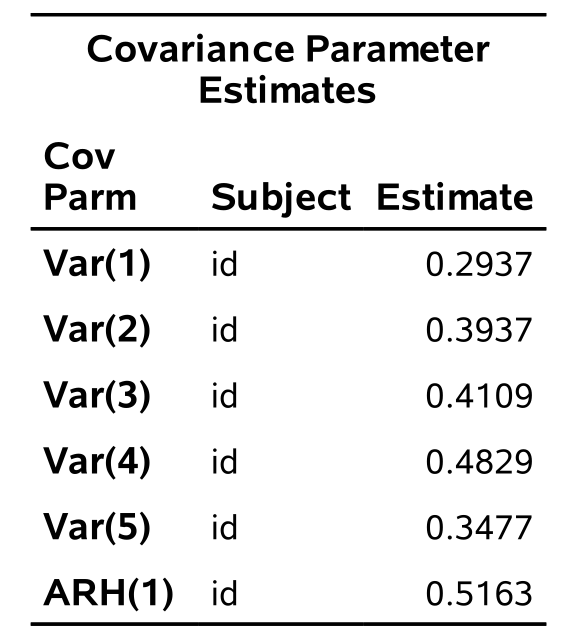
\includegraphics[width = 0.4\linewidth]{img/c5/slides6-e19}
\end{center}
\bi
\item This model includes six parameters in the covariance structure. 
\item In this table, we can see estimates of the variances of the five time points. 
\item The estimate for $\rho$ is $\hat{\rho}=0.516$, comparable to the estimate from the preceding model ($0.492$).
\ei 
\end{frame}



\begin{frame}[fragile]
\frametitle{Likelihood ratio test for $\mathsf{ARH}(1)$}
\begin{center}
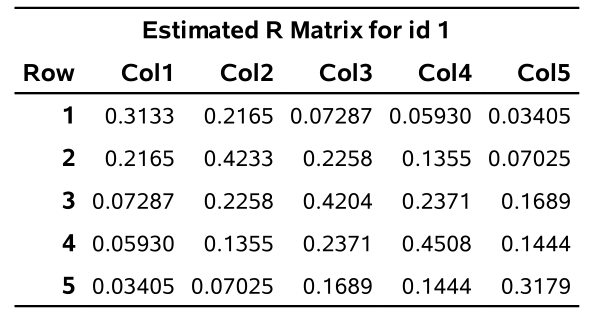
\includegraphics[width = 0.45\linewidth]{img/c5/slides6-e21a}
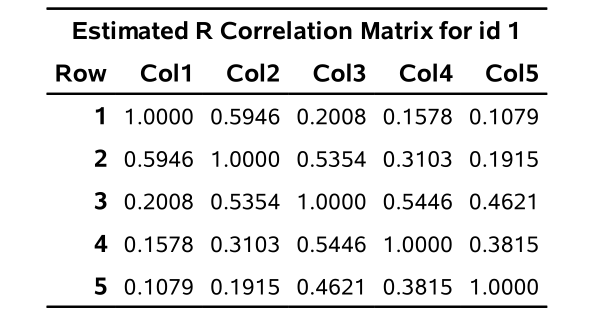
\includegraphics[width = 0.45\linewidth]{img/c5/slides6-e21b}
\end{center}
\bi
\item \SASlang{} outputs the results from the likelihood ratio test comparing the $\mathsf{ARH}(1)$ model (complete model) with a classical linear regression model with no correlation structure (reduced model).
\item The hypotheses are $\Hy_0: \rho=0, \sigma_1^2=\sigma_2^2=\cdots=\sigma_5^2$ and  $\Hy_1: \rho \neq 0$ or at least one variance differs.
\item The $p$-value is negligible, thus we can reject $\Hy_0$ and conclude in favour of the $\mathsf{ARH}(1)$ correlation structure.
\ei
\end{frame}

\begin{frame}[fragile]
\frametitle{Other possibilities for the choice of covariance structure}
\bi
\item Another possibility is not specifying any structure on the covariance,
\[
\bs{\Sigma}_i=
  \begin{pmatrix}
  \sigma^2_1 & \sigma_{12} & \sigma_{13} & \sigma_{14} & \sigma_{15} \\
   \sigma_{21} & \sigma_2^2  & \sigma_{23} & \sigma_{24} & \sigma_{25}\\
  \sigma_{31} & \sigma_{32} & \sigma^2_3 & \sigma_{34} & \sigma_{35}\\
   \sigma_{41} & \sigma_{42} & \sigma_{43} & \sigma_{4}^2 & \sigma_{45}\\
    \sigma_{51} & \sigma_{52} & \sigma_{53} & \sigma_{54}^2 & \sigma_{5}^2\\
    \end{pmatrix}
\]

\item This kind of structure can often be used to explore the covariance structure without
imposing any specific restrictions. We can only use this structure when the number of observations in each group is small and the number of groups is large, because it has $n \times(n+1)/2$ parameters.
\item In our example, we get $15$ parameters, compared to two parameters for the compound symmetry and the $\mathsf{AR}(1)$ covariance models, and
to six for the  $\mathsf{ARH}(1)$ covariance model. 

\ei
\end{frame}

\begin{frame}[fragile]
\frametitle{Unstructured covariance model}
 
\begin{tcolorbox}[colback=white, colframe=hecblue, title=\SASlang{} code to adjust an unstructure covariance model]
\begin{verbatim}
proc mixed data=revenge method=reml;
class id tcat;
model revenge = sex age vc wom t / solution;
repeated tcat / subject=id type=un r=1 rcorr=1;
run;
\end{verbatim}
\end{tcolorbox}
\end{frame}

\begin{frame}[fragile]
\frametitle{Estimated correlation and covariance matrices for subject 1}
\begin{center}
%\includegraphics[scale=0.35]{Figures/long34.pdf}
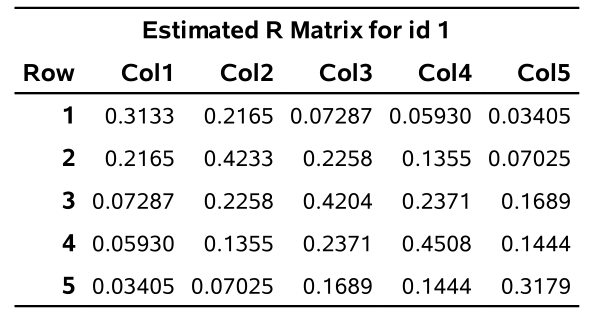
\includegraphics[width = 0.45\linewidth]{img/c5/slides6-e21a}
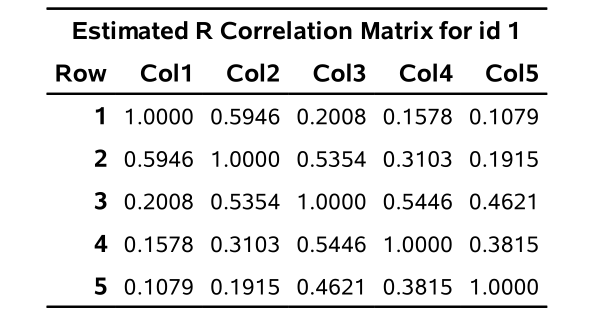
\includegraphics[width = 0.45\linewidth]{img/c5/slides6-e21b}
\end{center}
\bi
\item The variances are different for each time point, and there is no specific structure for the correlations.
\be

\item The estimated variances are very similar for all five time points. 
\item The estimated correlations between observations seems to decrease as the time between measurements increases. 
\ee
\item This would suggest that the $\mathsf{AR}(1)$ structure is preferable to the compound symmetry structure.
\ei
\end{frame}

\begin{frame}
\frametitle{Estimates of the unstructured covariance parameters }
\begin{center}
%\includegraphics[scale=0.35]{Figures/long36.pdf}
% \includegraphics[scale=0.3]{Figures/long37.pdf}
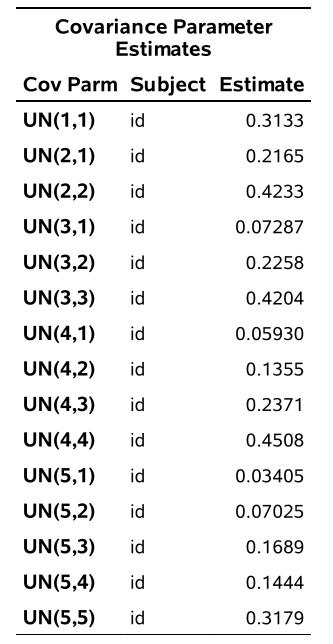
\includegraphics[width = 0.35\linewidth]{img/c5/slides6-e22}
\end{center}
% {\footnotesize Omitted output includes information criteria, parameter estimates for $\bs{\beta}$, likelihood ratio test,\ldots}

\end{frame}
\begin{frame}
\frametitle{Information criteria and likelihood ratio test}
\begin{center}
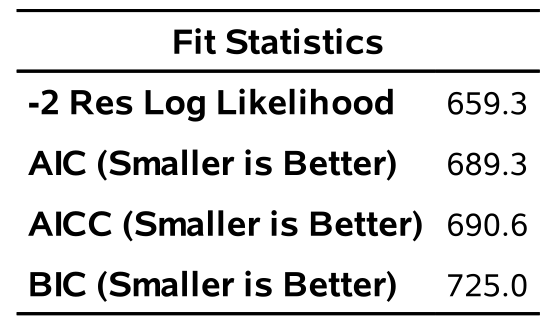
\includegraphics[width = 0.4\linewidth]{img/c5/slides6-e23}
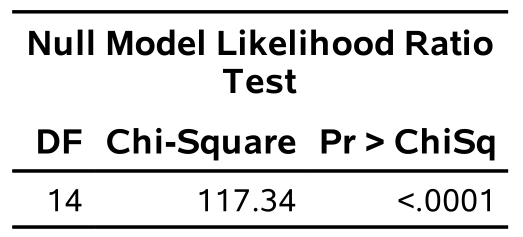
\includegraphics[width = 0.4\linewidth]{img/c5/slides6-e24}

\end{center}
\bi
\item As before, the AIC and BIC can be used to compare models with different correlation structures
\item The likelihood ratio tests the hypothesis that the model with independent homoscedastic observations for the group, with $\sigma^2$ for all diagonal elements and zero elsewhere is adequate. The hypothesis is soundly rejected.
\ei
\end{frame}
\end{document}
